% Options for packages loaded elsewhere
\PassOptionsToPackage{unicode}{hyperref}
\PassOptionsToPackage{hyphens}{url}
%
\documentclass[
]{article}
\usepackage{amsmath,amssymb}
\usepackage{iftex}
\ifPDFTeX
  \usepackage[T1]{fontenc}
  \usepackage[utf8]{inputenc}
  \usepackage{textcomp} % provide euro and other symbols
\else % if luatex or xetex
  \usepackage{unicode-math} % this also loads fontspec
  \defaultfontfeatures{Scale=MatchLowercase}
  \defaultfontfeatures[\rmfamily]{Ligatures=TeX,Scale=1}
\fi
\usepackage{lmodern}
\ifPDFTeX\else
  % xetex/luatex font selection
\fi
% Use upquote if available, for straight quotes in verbatim environments
\IfFileExists{upquote.sty}{\usepackage{upquote}}{}
\IfFileExists{microtype.sty}{% use microtype if available
  \usepackage[]{microtype}
  \UseMicrotypeSet[protrusion]{basicmath} % disable protrusion for tt fonts
}{}
\makeatletter
\@ifundefined{KOMAClassName}{% if non-KOMA class
  \IfFileExists{parskip.sty}{%
    \usepackage{parskip}
  }{% else
    \setlength{\parindent}{0pt}
    \setlength{\parskip}{6pt plus 2pt minus 1pt}}
}{% if KOMA class
  \KOMAoptions{parskip=half}}
\makeatother
\usepackage{xcolor}
\usepackage[margin=1in]{geometry}
\usepackage{color}
\usepackage{fancyvrb}
\newcommand{\VerbBar}{|}
\newcommand{\VERB}{\Verb[commandchars=\\\{\}]}
\DefineVerbatimEnvironment{Highlighting}{Verbatim}{commandchars=\\\{\}}
% Add ',fontsize=\small' for more characters per line
\usepackage{framed}
\definecolor{shadecolor}{RGB}{248,248,248}
\newenvironment{Shaded}{\begin{snugshade}}{\end{snugshade}}
\newcommand{\AlertTok}[1]{\textcolor[rgb]{0.94,0.16,0.16}{#1}}
\newcommand{\AnnotationTok}[1]{\textcolor[rgb]{0.56,0.35,0.01}{\textbf{\textit{#1}}}}
\newcommand{\AttributeTok}[1]{\textcolor[rgb]{0.13,0.29,0.53}{#1}}
\newcommand{\BaseNTok}[1]{\textcolor[rgb]{0.00,0.00,0.81}{#1}}
\newcommand{\BuiltInTok}[1]{#1}
\newcommand{\CharTok}[1]{\textcolor[rgb]{0.31,0.60,0.02}{#1}}
\newcommand{\CommentTok}[1]{\textcolor[rgb]{0.56,0.35,0.01}{\textit{#1}}}
\newcommand{\CommentVarTok}[1]{\textcolor[rgb]{0.56,0.35,0.01}{\textbf{\textit{#1}}}}
\newcommand{\ConstantTok}[1]{\textcolor[rgb]{0.56,0.35,0.01}{#1}}
\newcommand{\ControlFlowTok}[1]{\textcolor[rgb]{0.13,0.29,0.53}{\textbf{#1}}}
\newcommand{\DataTypeTok}[1]{\textcolor[rgb]{0.13,0.29,0.53}{#1}}
\newcommand{\DecValTok}[1]{\textcolor[rgb]{0.00,0.00,0.81}{#1}}
\newcommand{\DocumentationTok}[1]{\textcolor[rgb]{0.56,0.35,0.01}{\textbf{\textit{#1}}}}
\newcommand{\ErrorTok}[1]{\textcolor[rgb]{0.64,0.00,0.00}{\textbf{#1}}}
\newcommand{\ExtensionTok}[1]{#1}
\newcommand{\FloatTok}[1]{\textcolor[rgb]{0.00,0.00,0.81}{#1}}
\newcommand{\FunctionTok}[1]{\textcolor[rgb]{0.13,0.29,0.53}{\textbf{#1}}}
\newcommand{\ImportTok}[1]{#1}
\newcommand{\InformationTok}[1]{\textcolor[rgb]{0.56,0.35,0.01}{\textbf{\textit{#1}}}}
\newcommand{\KeywordTok}[1]{\textcolor[rgb]{0.13,0.29,0.53}{\textbf{#1}}}
\newcommand{\NormalTok}[1]{#1}
\newcommand{\OperatorTok}[1]{\textcolor[rgb]{0.81,0.36,0.00}{\textbf{#1}}}
\newcommand{\OtherTok}[1]{\textcolor[rgb]{0.56,0.35,0.01}{#1}}
\newcommand{\PreprocessorTok}[1]{\textcolor[rgb]{0.56,0.35,0.01}{\textit{#1}}}
\newcommand{\RegionMarkerTok}[1]{#1}
\newcommand{\SpecialCharTok}[1]{\textcolor[rgb]{0.81,0.36,0.00}{\textbf{#1}}}
\newcommand{\SpecialStringTok}[1]{\textcolor[rgb]{0.31,0.60,0.02}{#1}}
\newcommand{\StringTok}[1]{\textcolor[rgb]{0.31,0.60,0.02}{#1}}
\newcommand{\VariableTok}[1]{\textcolor[rgb]{0.00,0.00,0.00}{#1}}
\newcommand{\VerbatimStringTok}[1]{\textcolor[rgb]{0.31,0.60,0.02}{#1}}
\newcommand{\WarningTok}[1]{\textcolor[rgb]{0.56,0.35,0.01}{\textbf{\textit{#1}}}}
\usepackage{graphicx}
\makeatletter
\def\maxwidth{\ifdim\Gin@nat@width>\linewidth\linewidth\else\Gin@nat@width\fi}
\def\maxheight{\ifdim\Gin@nat@height>\textheight\textheight\else\Gin@nat@height\fi}
\makeatother
% Scale images if necessary, so that they will not overflow the page
% margins by default, and it is still possible to overwrite the defaults
% using explicit options in \includegraphics[width, height, ...]{}
\setkeys{Gin}{width=\maxwidth,height=\maxheight,keepaspectratio}
% Set default figure placement to htbp
\makeatletter
\def\fps@figure{htbp}
\makeatother
\setlength{\emergencystretch}{3em} % prevent overfull lines
\providecommand{\tightlist}{%
  \setlength{\itemsep}{0pt}\setlength{\parskip}{0pt}}
\setcounter{secnumdepth}{-\maxdimen} % remove section numbering
\usepackage{booktabs}
\usepackage{longtable}
\usepackage{array}
\usepackage{multirow}
\usepackage{wrapfig}
\usepackage{float}
\usepackage{colortbl}
\usepackage{pdflscape}
\usepackage{tabu}
\usepackage{threeparttable}
\usepackage{threeparttablex}
\usepackage[normalem]{ulem}
\usepackage{makecell}
\usepackage{xcolor}
\ifLuaTeX
  \usepackage{selnolig}  % disable illegal ligatures
\fi
\IfFileExists{bookmark.sty}{\usepackage{bookmark}}{\usepackage{hyperref}}
\IfFileExists{xurl.sty}{\usepackage{xurl}}{} % add URL line breaks if available
\urlstyle{same}
\hypersetup{
  pdftitle={Homework \#1 Assignment Requirements},
  pdfauthor={Warner Alexis},
  hidelinks,
  pdfcreator={LaTeX via pandoc}}

\title{Homework \#1 Assignment Requirements}
\author{Warner Alexis}
\date{2024-09-17}

\begin{document}
\maketitle

\hypertarget{introduction}{%
\subsection{Introduction}\label{introduction}}

In this assignment, I will be exploring, analyzing and modeing the
\textbf{money ball dataset}. Each record represents a professional
baseball team from the years 1871 to 2006 inclusive. Each record has the
performance of the team for the given year, with all of the statistics
adjusted to match the performance of a 162 game season. the purpose of
this assignment is to build a multiple linear regression model on the
training data to predict the number of wins for the team.

\hypertarget{descriptive-analysis}{%
\subsection{Descriptive Analysis}\label{descriptive-analysis}}

\begin{quote}
Variables:
\end{quote}

\textbf{INDEX} Identification Variable (do not use)

\textbf{TARGET\_WINS} Number of wins

\textbf{TEAM\_BATTING\_H} Base Hits by batters (1B,2B,3B,HR)

\textbf{TEAM\_BATTING\_2B} Doubles by batters (2B)

\textbf{TEAM\_BATTING\_3B} Triples by batters (3B)

\textbf{TEAM\_BATTING\_HR} Homeruns by batters (4B)

\textbf{TEAM\_BATTING\_BB} Walks by batters Positive

\textbf{TEAM\_BATTING\_HBP} Batters hit by pitch (get a free base)

\textbf{TEAM\_BATTING\_SO} Strikeouts by batters

\textbf{TEAM\_BASERUN\_SB} Stolen bases

\textbf{TEAM\_BASERUN\_CS} Caught stealing

\textbf{TEAM\_FIELDING\_E} Errors

\textbf{TEAM\_FIELDING\_DP} Double Plays

\textbf{TEAM\_PITCHING\_BB} Walks allowed

\textbf{TEAM\_PITCHING\_H} Hits allowed

\textbf{TEAM\_PITCHING\_HR} Homeruns allowed

\textbf{TEAM\_PITCHING\_SO} Strikeouts by pitchers

\begin{Shaded}
\begin{Highlighting}[]
\CommentTok{\# Loading library}
\FunctionTok{library}\NormalTok{(tidyverse)}
\end{Highlighting}
\end{Shaded}

\begin{verbatim}
## -- Attaching core tidyverse packages ------------------------ tidyverse 2.0.0 --
## v dplyr     1.1.4     v readr     2.1.5
## v forcats   1.0.0     v stringr   1.5.1
## v ggplot2   3.5.1     v tibble    3.2.1
## v lubridate 1.9.3     v tidyr     1.3.1
## v purrr     1.0.2     
## -- Conflicts ------------------------------------------ tidyverse_conflicts() --
## x dplyr::filter() masks stats::filter()
## x dplyr::lag()    masks stats::lag()
## i Use the conflicted package (<http://conflicted.r-lib.org/>) to force all conflicts to become errors
\end{verbatim}

\begin{Shaded}
\begin{Highlighting}[]
\FunctionTok{library}\NormalTok{(ggplot2)}
\FunctionTok{library}\NormalTok{(DataExplorer)}
\FunctionTok{library}\NormalTok{(mice)}
\end{Highlighting}
\end{Shaded}

\begin{verbatim}
## 
## Attaching package: 'mice'
## 
## The following object is masked from 'package:stats':
## 
##     filter
## 
## The following objects are masked from 'package:base':
## 
##     cbind, rbind
\end{verbatim}

\begin{Shaded}
\begin{Highlighting}[]
\FunctionTok{library}\NormalTok{(kableExtra)}
\end{Highlighting}
\end{Shaded}

\begin{verbatim}
## 
## Attaching package: 'kableExtra'
## 
## The following object is masked from 'package:dplyr':
## 
##     group_rows
\end{verbatim}

\begin{Shaded}
\begin{Highlighting}[]
\FunctionTok{library}\NormalTok{(corrplot)}
\end{Highlighting}
\end{Shaded}

\begin{verbatim}
## corrplot 0.94 loaded
\end{verbatim}

\begin{Shaded}
\begin{Highlighting}[]
\FunctionTok{library}\NormalTok{(reshape)}
\end{Highlighting}
\end{Shaded}

\begin{verbatim}
## 
## Attaching package: 'reshape'
## 
## The following object is masked from 'package:lubridate':
## 
##     stamp
## 
## The following object is masked from 'package:dplyr':
## 
##     rename
## 
## The following objects are masked from 'package:tidyr':
## 
##     expand, smiths
\end{verbatim}

\begin{Shaded}
\begin{Highlighting}[]
\FunctionTok{library}\NormalTok{(reshape2)}
\end{Highlighting}
\end{Shaded}

\begin{verbatim}
## 
## Attaching package: 'reshape2'
## 
## The following objects are masked from 'package:reshape':
## 
##     colsplit, melt, recast
## 
## The following object is masked from 'package:tidyr':
## 
##     smiths
\end{verbatim}

\begin{Shaded}
\begin{Highlighting}[]
\FunctionTok{library}\NormalTok{(caret)}
\end{Highlighting}
\end{Shaded}

\begin{verbatim}
## Loading required package: lattice
## 
## Attaching package: 'caret'
## 
## The following object is masked from 'package:purrr':
## 
##     lift
\end{verbatim}

\begin{Shaded}
\begin{Highlighting}[]
\FunctionTok{library}\NormalTok{(dplyr)}
\FunctionTok{library}\NormalTok{(factoextra)}
\end{Highlighting}
\end{Shaded}

\begin{verbatim}
## Welcome! Want to learn more? See two factoextra-related books at https://goo.gl/ve3WBa
\end{verbatim}

\begin{Shaded}
\begin{Highlighting}[]
\FunctionTok{library}\NormalTok{(caret)  }\CommentTok{\# for data splitting and pre{-}processing}
\FunctionTok{library}\NormalTok{(stats) }
\end{Highlighting}
\end{Shaded}

we have two data sets: -** a training set : where most analysis will be
doing -** A evaluation set Which will be used to evaluate the model

\begin{Shaded}
\begin{Highlighting}[]
\CommentTok{\# load data money ball }
\CommentTok{\#evaluation set use for test set }
\NormalTok{money\_ball\_eval }\OtherTok{\textless{}{-}} \FunctionTok{read.csv}\NormalTok{(}\StringTok{\textquotesingle{}moneyball{-}evaluation{-}data.csv\textquotesingle{}}\NormalTok{)}
\CommentTok{\# training  set }
\NormalTok{money\_ball\_train }\OtherTok{\textless{}{-}} \FunctionTok{read.csv}\NormalTok{(}\StringTok{\textquotesingle{}moneyball{-}training{-}data.csv\textquotesingle{}}\NormalTok{)}
\FunctionTok{str}\NormalTok{(money\_ball\_train)}
\end{Highlighting}
\end{Shaded}

\begin{verbatim}
## 'data.frame':    2276 obs. of  17 variables:
##  $ INDEX           : int  1 2 3 4 5 6 7 8 11 12 ...
##  $ TARGET_WINS     : int  39 70 86 70 82 75 80 85 86 76 ...
##  $ TEAM_BATTING_H  : int  1445 1339 1377 1387 1297 1279 1244 1273 1391 1271 ...
##  $ TEAM_BATTING_2B : int  194 219 232 209 186 200 179 171 197 213 ...
##  $ TEAM_BATTING_3B : int  39 22 35 38 27 36 54 37 40 18 ...
##  $ TEAM_BATTING_HR : int  13 190 137 96 102 92 122 115 114 96 ...
##  $ TEAM_BATTING_BB : int  143 685 602 451 472 443 525 456 447 441 ...
##  $ TEAM_BATTING_SO : int  842 1075 917 922 920 973 1062 1027 922 827 ...
##  $ TEAM_BASERUN_SB : int  NA 37 46 43 49 107 80 40 69 72 ...
##  $ TEAM_BASERUN_CS : int  NA 28 27 30 39 59 54 36 27 34 ...
##  $ TEAM_BATTING_HBP: int  NA NA NA NA NA NA NA NA NA NA ...
##  $ TEAM_PITCHING_H : int  9364 1347 1377 1396 1297 1279 1244 1281 1391 1271 ...
##  $ TEAM_PITCHING_HR: int  84 191 137 97 102 92 122 116 114 96 ...
##  $ TEAM_PITCHING_BB: int  927 689 602 454 472 443 525 459 447 441 ...
##  $ TEAM_PITCHING_SO: int  5456 1082 917 928 920 973 1062 1033 922 827 ...
##  $ TEAM_FIELDING_E : int  1011 193 175 164 138 123 136 112 127 131 ...
##  $ TEAM_FIELDING_DP: int  NA 155 153 156 168 149 186 136 169 159 ...
\end{verbatim}

\begin{Shaded}
\begin{Highlighting}[]
\FunctionTok{introduce}\NormalTok{(money\_ball\_train)}
\end{Highlighting}
\end{Shaded}

\begin{verbatim}
##   rows columns discrete_columns continuous_columns all_missing_columns
## 1 2276      17                0                 17                   0
##   total_missing_values complete_rows total_observations memory_usage
## 1                 3478           191              38692       159280
\end{verbatim}

\begin{Shaded}
\begin{Highlighting}[]
\CommentTok{\# Data Description }
\NormalTok{money\_ball\_train }\SpecialCharTok{\%\textgreater{}\%} 
  \FunctionTok{summary}\NormalTok{() }\SpecialCharTok{\%\textgreater{}\%}
  \FunctionTok{kable}\NormalTok{() }\SpecialCharTok{\%\textgreater{}\%} \FunctionTok{kable\_styling}\NormalTok{() }\SpecialCharTok{\%\textgreater{}\%}  \FunctionTok{kable\_classic}\NormalTok{(}\AttributeTok{full\_width =}\NormalTok{ F, }\AttributeTok{html\_font =} \StringTok{"Cambria"}\NormalTok{)}
\end{Highlighting}
\end{Shaded}

\begin{longtable}[t]{llllllllllllllllll}
\toprule
 & INDEX & TARGET\_WINS & TEAM\_BATTING\_H & TEAM\_BATTING\_2B & TEAM\_BATTING\_3B & TEAM\_BATTING\_HR & TEAM\_BATTING\_BB & TEAM\_BATTING\_SO & TEAM\_BASERUN\_SB & TEAM\_BASERUN\_CS & TEAM\_BATTING\_HBP & TEAM\_PITCHING\_H & TEAM\_PITCHING\_HR & TEAM\_PITCHING\_BB & TEAM\_PITCHING\_SO & TEAM\_FIELDING\_E & TEAM\_FIELDING\_DP\\
\midrule
 & Min.   :   1.0 & Min.   :  0.00 & Min.   : 891 & Min.   : 69.0 & Min.   :  0.00 & Min.   :  0.00 & Min.   :  0.0 & Min.   :   0.0 & Min.   :  0.0 & Min.   :  0.0 & Min.   :29.00 & Min.   : 1137 & Min.   :  0.0 & Min.   :   0.0 & Min.   :    0.0 & Min.   :  65.0 & Min.   : 52.0\\
 & 1st Qu.: 630.8 & 1st Qu.: 71.00 & 1st Qu.:1383 & 1st Qu.:208.0 & 1st Qu.: 34.00 & 1st Qu.: 42.00 & 1st Qu.:451.0 & 1st Qu.: 548.0 & 1st Qu.: 66.0 & 1st Qu.: 38.0 & 1st Qu.:50.50 & 1st Qu.: 1419 & 1st Qu.: 50.0 & 1st Qu.: 476.0 & 1st Qu.:  615.0 & 1st Qu.: 127.0 & 1st Qu.:131.0\\
 & Median :1270.5 & Median : 82.00 & Median :1454 & Median :238.0 & Median : 47.00 & Median :102.00 & Median :512.0 & Median : 750.0 & Median :101.0 & Median : 49.0 & Median :58.00 & Median : 1518 & Median :107.0 & Median : 536.5 & Median :  813.5 & Median : 159.0 & Median :149.0\\
 & Mean   :1268.5 & Mean   : 80.79 & Mean   :1469 & Mean   :241.2 & Mean   : 55.25 & Mean   : 99.61 & Mean   :501.6 & Mean   : 735.6 & Mean   :124.8 & Mean   : 52.8 & Mean   :59.36 & Mean   : 1779 & Mean   :105.7 & Mean   : 553.0 & Mean   :  817.7 & Mean   : 246.5 & Mean   :146.4\\
 & 3rd Qu.:1915.5 & 3rd Qu.: 92.00 & 3rd Qu.:1537 & 3rd Qu.:273.0 & 3rd Qu.: 72.00 & 3rd Qu.:147.00 & 3rd Qu.:580.0 & 3rd Qu.: 930.0 & 3rd Qu.:156.0 & 3rd Qu.: 62.0 & 3rd Qu.:67.00 & 3rd Qu.: 1682 & 3rd Qu.:150.0 & 3rd Qu.: 611.0 & 3rd Qu.:  968.0 & 3rd Qu.: 249.2 & 3rd Qu.:164.0\\
\addlinespace
 & Max.   :2535.0 & Max.   :146.00 & Max.   :2554 & Max.   :458.0 & Max.   :223.00 & Max.   :264.00 & Max.   :878.0 & Max.   :1399.0 & Max.   :697.0 & Max.   :201.0 & Max.   :95.00 & Max.   :30132 & Max.   :343.0 & Max.   :3645.0 & Max.   :19278.0 & Max.   :1898.0 & Max.   :228.0\\
 & NA & NA & NA & NA & NA & NA & NA & NA's   :102 & NA's   :131 & NA's   :772 & NA's   :2085 & NA & NA & NA & NA's   :102 & NA & NA's   :286\\
\bottomrule
\end{longtable}

\begin{Shaded}
\begin{Highlighting}[]
\FunctionTok{str}\NormalTok{(money\_ball\_train)}
\end{Highlighting}
\end{Shaded}

\begin{verbatim}
## 'data.frame':    2276 obs. of  17 variables:
##  $ INDEX           : int  1 2 3 4 5 6 7 8 11 12 ...
##  $ TARGET_WINS     : int  39 70 86 70 82 75 80 85 86 76 ...
##  $ TEAM_BATTING_H  : int  1445 1339 1377 1387 1297 1279 1244 1273 1391 1271 ...
##  $ TEAM_BATTING_2B : int  194 219 232 209 186 200 179 171 197 213 ...
##  $ TEAM_BATTING_3B : int  39 22 35 38 27 36 54 37 40 18 ...
##  $ TEAM_BATTING_HR : int  13 190 137 96 102 92 122 115 114 96 ...
##  $ TEAM_BATTING_BB : int  143 685 602 451 472 443 525 456 447 441 ...
##  $ TEAM_BATTING_SO : int  842 1075 917 922 920 973 1062 1027 922 827 ...
##  $ TEAM_BASERUN_SB : int  NA 37 46 43 49 107 80 40 69 72 ...
##  $ TEAM_BASERUN_CS : int  NA 28 27 30 39 59 54 36 27 34 ...
##  $ TEAM_BATTING_HBP: int  NA NA NA NA NA NA NA NA NA NA ...
##  $ TEAM_PITCHING_H : int  9364 1347 1377 1396 1297 1279 1244 1281 1391 1271 ...
##  $ TEAM_PITCHING_HR: int  84 191 137 97 102 92 122 116 114 96 ...
##  $ TEAM_PITCHING_BB: int  927 689 602 454 472 443 525 459 447 441 ...
##  $ TEAM_PITCHING_SO: int  5456 1082 917 928 920 973 1062 1033 922 827 ...
##  $ TEAM_FIELDING_E : int  1011 193 175 164 138 123 136 112 127 131 ...
##  $ TEAM_FIELDING_DP: int  NA 155 153 156 168 149 186 136 169 159 ...
\end{verbatim}

\hypertarget{data-preparation}{%
\subsection{Data Preparation}\label{data-preparation}}

We are going to check distribution for all the columns and outliers that
are present in the data set. The Chart below shows the percentage
accounted for missing values in the data set. We notice that
TEAM\_BATTING\_HBP has the highest number of missing values but, the
mean, the median, the max are around the same rangle which mean that
column is skewed centerely.

\begin{Shaded}
\begin{Highlighting}[]
\CommentTok{\# Correlation Plot}
\NormalTok{cor\_matrix }\OtherTok{\textless{}{-}} \FunctionTok{cor}\NormalTok{(money\_ball\_train, }\AttributeTok{use =} \StringTok{\textquotesingle{}complete.obs\textquotesingle{}}\NormalTok{)}
\FunctionTok{corrplot}\NormalTok{(cor\_matrix, }\AttributeTok{method =} \StringTok{\textquotesingle{}circle\textquotesingle{}}\NormalTok{)}
\end{Highlighting}
\end{Shaded}

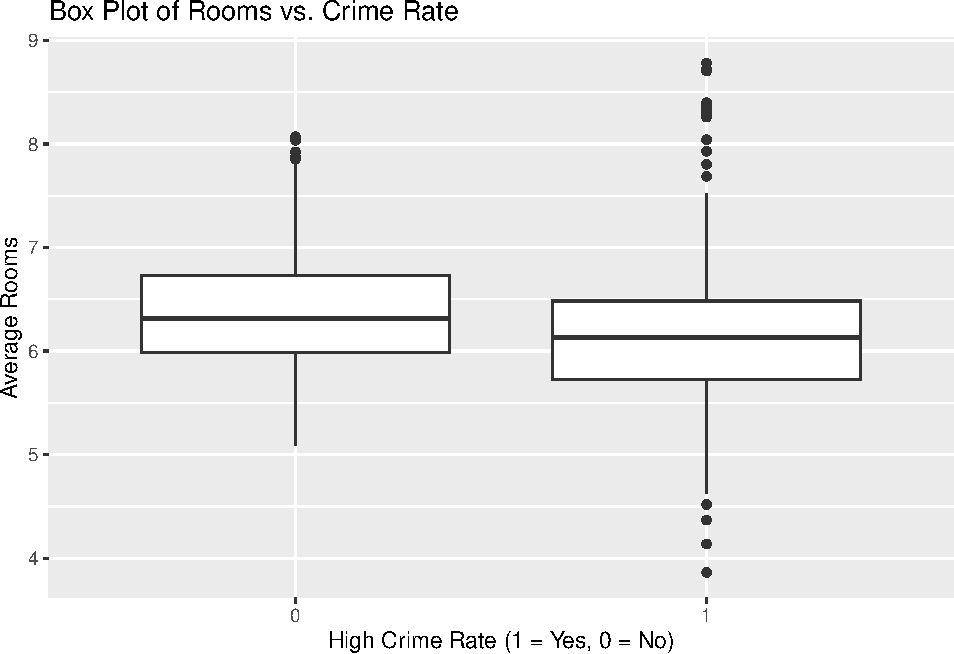
\includegraphics{Homework--1-Assignment-Requirements_files/figure-latex/unnamed-chunk-3-1.pdf}

\begin{Shaded}
\begin{Highlighting}[]
\NormalTok{money }\OtherTok{\textless{}{-}}\NormalTok{ money\_ball\_train}
\CommentTok{\# Create missing data flags}

\CommentTok{\# Create missing data flags}
\CommentTok{\#missing\_flag \textless{}{-} ifelse(is.na(money\_ball\_train$TEAM\_BATTING\_HBP), 1, 2)}
\CommentTok{\#money\_ball\_train$missing\_flag \textless{}{-} missing\_flag}


\FunctionTok{par}\NormalTok{(}\AttributeTok{mfrow=}\FunctionTok{c}\NormalTok{(}\DecValTok{3}\NormalTok{,}\DecValTok{3}\NormalTok{)) }
\CommentTok{\# Create distribution plot to check outliers }
\ControlFlowTok{for}\NormalTok{ (i }\ControlFlowTok{in} \DecValTok{1}\SpecialCharTok{:}\DecValTok{17}\NormalTok{) \{}
  \FunctionTok{hist}\NormalTok{(money[,i],}\AttributeTok{main=}\FunctionTok{names}\NormalTok{(money[i]),}\AttributeTok{xlab=}\FunctionTok{names}\NormalTok{(money[i]),}\AttributeTok{breaks =} \DecValTok{51}\NormalTok{)}
  \FunctionTok{boxplot}\NormalTok{(money[,i], }\AttributeTok{main=}\FunctionTok{names}\NormalTok{(money[i]), }\AttributeTok{type=}\StringTok{"l"}\NormalTok{,}\AttributeTok{horizontal =} \ConstantTok{TRUE}\NormalTok{)}
  
  \FunctionTok{plot}\NormalTok{(money[,i], money}\SpecialCharTok{$}\NormalTok{TARGET\_WINS, }\AttributeTok{main =} \FunctionTok{names}\NormalTok{(money[i]), }\AttributeTok{xlab=}\FunctionTok{names}\NormalTok{(money[i]))}
  \FunctionTok{abline}\NormalTok{(}\FunctionTok{lm}\NormalTok{(money}\SpecialCharTok{$}\NormalTok{TARGET\_WINS }\SpecialCharTok{\textasciitilde{}}\NormalTok{ money[,i], }\AttributeTok{data =}\NormalTok{ money), }\AttributeTok{col =} \StringTok{"blue"}\NormalTok{)}
\NormalTok{\}}
\end{Highlighting}
\end{Shaded}

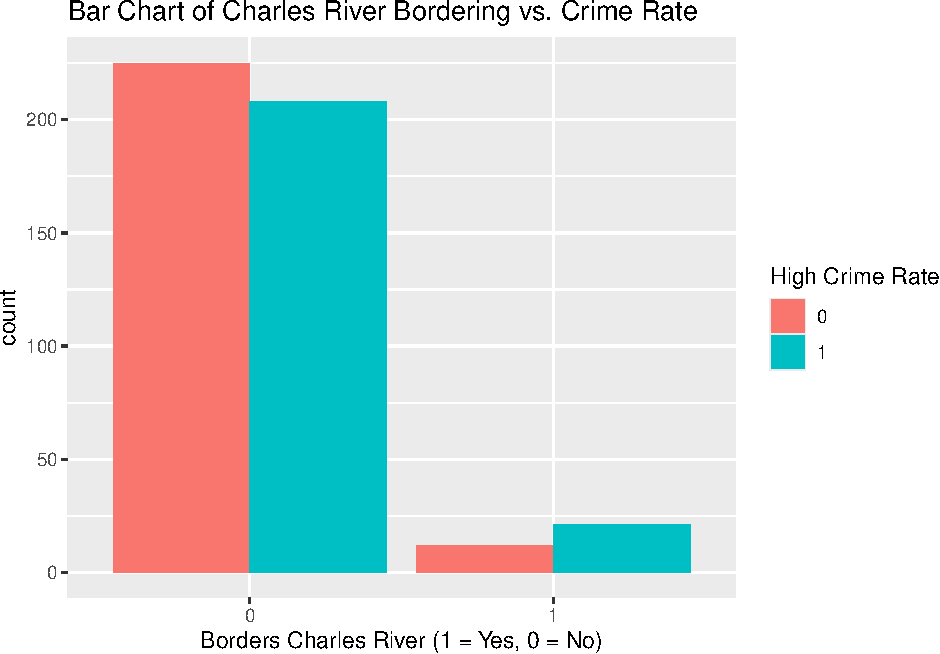
\includegraphics{Homework--1-Assignment-Requirements_files/figure-latex/unnamed-chunk-3-2.pdf}
\includegraphics{Homework--1-Assignment-Requirements_files/figure-latex/unnamed-chunk-3-3.pdf}
\includegraphics{Homework--1-Assignment-Requirements_files/figure-latex/unnamed-chunk-3-4.pdf}
\includegraphics{Homework--1-Assignment-Requirements_files/figure-latex/unnamed-chunk-3-5.pdf}
\includegraphics{Homework--1-Assignment-Requirements_files/figure-latex/unnamed-chunk-3-6.pdf}
\includegraphics{Homework--1-Assignment-Requirements_files/figure-latex/unnamed-chunk-3-7.pdf}

The relationship between the target variable and the predictors is not
particularly strong, but there are statistically significant
relationships with certain variables. The
calculate\_correlations\_with\_pvalues function computes the correlation
coefficients and p-values between a given target variable and all other
predictor variables in a dataset. It first validates the input to ensure
that the target variable is present and that the data contains no
missing values. For each predictor, the function performs a correlation
test using cor.test(), which returns both the correlation coefficient
and the corresponding p-value. These results are stored in a data frame,
with both the correlation and p-value rounded to 10 decimal places for
precision. This function offers a clear, organized output, making it
easy for users to evaluate the strength and statistical significance of
the relationships between the target variable and the predictors.

\begin{Shaded}
\begin{Highlighting}[]
\NormalTok{calculate\_correlations\_with\_pvalues }\OtherTok{\textless{}{-}} \ControlFlowTok{function}\NormalTok{(data, target\_col) \{}
  \CommentTok{\# Check if target\_col is a character string}
  \ControlFlowTok{if}\NormalTok{ (}\SpecialCharTok{!}\FunctionTok{is.character}\NormalTok{(target\_col) }\SpecialCharTok{||} \FunctionTok{length}\NormalTok{(target\_col) }\SpecialCharTok{!=} \DecValTok{1}\NormalTok{) \{}
    \FunctionTok{stop}\NormalTok{(}\StringTok{"target\_col must be a single character string."}\NormalTok{)}
\NormalTok{  \}}
  
  \CommentTok{\# Ensure the target column exists in the data}
  \ControlFlowTok{if}\NormalTok{ (}\SpecialCharTok{!}\NormalTok{target\_col }\SpecialCharTok{\%in\%} \FunctionTok{names}\NormalTok{(data)) \{}
    \FunctionTok{stop}\NormalTok{(}\StringTok{"Target column not found in the dataframe."}\NormalTok{)}
\NormalTok{  \}}
  
  \CommentTok{\# Remove rows with missing values}
\NormalTok{  data\_complete }\OtherTok{\textless{}{-}}\NormalTok{ data[}\FunctionTok{complete.cases}\NormalTok{(data), ]}
  
  \CommentTok{\# Initialize a results data frame}
\NormalTok{  results }\OtherTok{\textless{}{-}} \FunctionTok{data.frame}\NormalTok{(}\AttributeTok{Predictor =} \FunctionTok{character}\NormalTok{(), }\AttributeTok{Correlation =} \FunctionTok{numeric}\NormalTok{(), }\AttributeTok{PValue =} \FunctionTok{numeric}\NormalTok{(), }\AttributeTok{stringsAsFactors =} \ConstantTok{FALSE}\NormalTok{)}
  
  \CommentTok{\# Loop through each predictor variable}
  \ControlFlowTok{for}\NormalTok{ (predictor }\ControlFlowTok{in} \FunctionTok{names}\NormalTok{(data\_complete)[}\FunctionTok{names}\NormalTok{(data\_complete) }\SpecialCharTok{!=}\NormalTok{ target\_col]) \{}
    \CommentTok{\# Perform the correlation test}
\NormalTok{    test\_result }\OtherTok{\textless{}{-}} \FunctionTok{cor.test}\NormalTok{(data\_complete[[predictor]], data\_complete[[target\_col]])}
    
    \CommentTok{\# Store the rounded results to 10 decimal places}
\NormalTok{    results }\OtherTok{\textless{}{-}} \FunctionTok{rbind}\NormalTok{(results, }\FunctionTok{data.frame}\NormalTok{(}\AttributeTok{Predictor =}\NormalTok{ predictor, }
                                         \AttributeTok{Correlation =} \FunctionTok{round}\NormalTok{(test\_result}\SpecialCharTok{$}\NormalTok{estimate, }\DecValTok{10}\NormalTok{), }
                                         \AttributeTok{PValue =} \FunctionTok{round}\NormalTok{(test\_result}\SpecialCharTok{$}\NormalTok{p.value, }\DecValTok{10}\NormalTok{)))}
\NormalTok{  \}}
  
  \FunctionTok{return}\NormalTok{(results)}
\NormalTok{\}}


\CommentTok{\# Example usage}
\NormalTok{correlation\_results }\OtherTok{\textless{}{-}} \FunctionTok{calculate\_correlations\_with\_pvalues}\NormalTok{(money\_ball\_train, }\StringTok{"TARGET\_WINS"}\NormalTok{)}

\CommentTok{\# View the results}
\FunctionTok{print}\NormalTok{(correlation\_results)}
\end{Highlighting}
\end{Shaded}

\begin{verbatim}
##              Predictor Correlation       PValue
## cor              INDEX -0.04895047 0.5012836479
## cor1    TEAM_BATTING_H  0.46994665 0.0000000000
## cor2   TEAM_BATTING_2B  0.31298400 0.0000104138
## cor3   TEAM_BATTING_3B -0.12434586 0.0865523694
## cor4   TEAM_BATTING_HR  0.42241683 0.0000000012
## cor5   TEAM_BATTING_BB  0.46868793 0.0000000000
## cor6   TEAM_BATTING_SO -0.22889273 0.0014476066
## cor7   TEAM_BASERUN_SB  0.01483639 0.8385814774
## cor8   TEAM_BASERUN_CS -0.17875598 0.0133534492
## cor9  TEAM_BATTING_HBP  0.07350424 0.3122327101
## cor10  TEAM_PITCHING_H  0.47123431 0.0000000000
## cor11 TEAM_PITCHING_HR  0.42246683 0.0000000011
## cor12 TEAM_PITCHING_BB  0.46839882 0.0000000000
## cor13 TEAM_PITCHING_SO -0.22936481 0.0014142043
## cor14  TEAM_FIELDING_E -0.38668800 0.0000000329
## cor15 TEAM_FIELDING_DP -0.19586601 0.0066174528
\end{verbatim}

Now let dive into the Missing values.

\begin{Shaded}
\begin{Highlighting}[]
\CommentTok{\# }
\FunctionTok{plot\_intro}\NormalTok{(money\_ball\_train, }\AttributeTok{title =} \StringTok{\textquotesingle{}Missing Information on Meny Ball Dataset\textquotesingle{}}\NormalTok{,}
           \AttributeTok{ggtheme =} \FunctionTok{theme\_minimal}\NormalTok{())}
\end{Highlighting}
\end{Shaded}

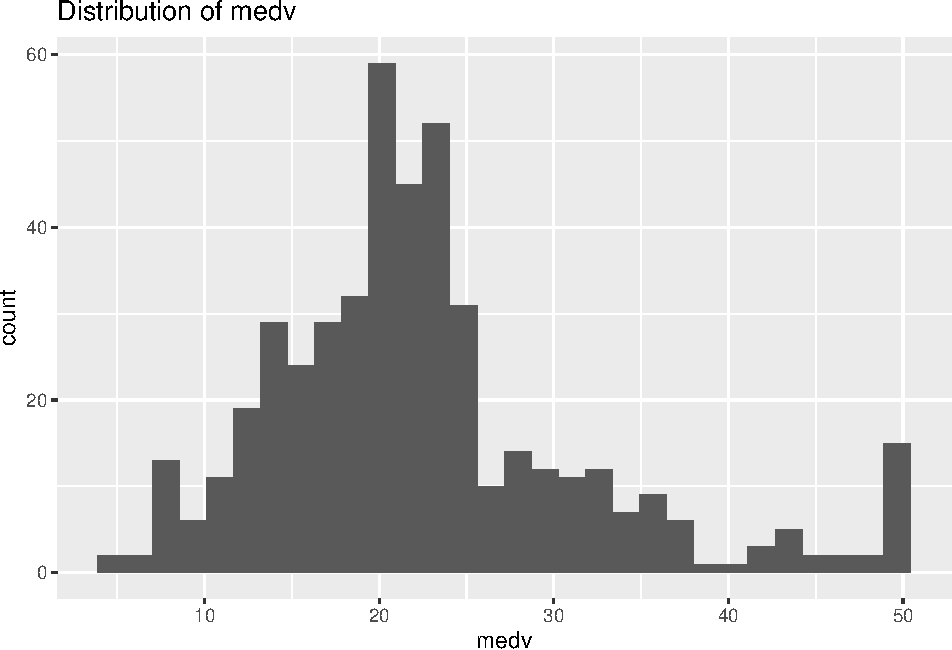
\includegraphics{Homework--1-Assignment-Requirements_files/figure-latex/unnamed-chunk-5-1.pdf}

\begin{Shaded}
\begin{Highlighting}[]
\CommentTok{\# Plot missing volume in Column }
\FunctionTok{plot\_missing}\NormalTok{(money\_ball\_train,}\AttributeTok{title =} \StringTok{\textquotesingle{}Information about Missing Value in money ball dataset\textquotesingle{}}\NormalTok{,}\AttributeTok{ggtheme =} \FunctionTok{theme\_minimal}\NormalTok{())}
\end{Highlighting}
\end{Shaded}

\includegraphics{Homework--1-Assignment-Requirements_files/figure-latex/unnamed-chunk-5-2.pdf}

we have discovered that there are some observations that are missing
data. These column names will need imputation after analysis. We have
about 9\% of the data missing that spread out to \textgreater{}
TEAM\_PITCHING\_SO 4.48\% \textgreater{} TEAM\_BATTING\_SO 4.48\%
\textgreater{} TEAM\_BASERUN\_SB 5.76\% \textgreater{} TEAM\_BASERUN\_CS
12.57\% \textgreater{} TEAM\_BATTING\_HBP 91.61\%

\textbf{Why Use Predictive Imputation?}

\textbf{Preserves Relationships}: Predictive imputation uses the
relationships between variables to estimate missing values, which can
lead to more accurate and reliable data sets.

\textbf{Handles Different Types of Missing Data}: It can handle data
that is Missing Completely at Random (MCAR), Missing at Random (MAR),
and even some cases of Missing Not at Random (MNAR). \textbf{Maintains
Variability}: Unlike simple imputation methods (mean, median),
predictive imputation maintains the natural variability in the data.

\begin{Shaded}
\begin{Highlighting}[]
\CommentTok{\# re{-}assign moneyball}
\NormalTok{money }\OtherTok{\textless{}{-}}\NormalTok{ money\_ball\_train}
\CommentTok{\# create data set with with predictive imputable }
\CommentTok{\# Compute multiple imputation }
\NormalTok{data1 }\OtherTok{\textless{}{-}} \FunctionTok{mice}\NormalTok{(money, }\AttributeTok{method =} \StringTok{\textquotesingle{}pmm\textquotesingle{}}\NormalTok{, }\AttributeTok{m=}\DecValTok{5}\NormalTok{)}
\end{Highlighting}
\end{Shaded}

\begin{verbatim}
## 
##  iter imp variable
##   1   1  TEAM_BATTING_SO  TEAM_BASERUN_SB  TEAM_BASERUN_CS  TEAM_BATTING_HBP  TEAM_PITCHING_SO  TEAM_FIELDING_DP
##   1   2  TEAM_BATTING_SO  TEAM_BASERUN_SB  TEAM_BASERUN_CS  TEAM_BATTING_HBP  TEAM_PITCHING_SO  TEAM_FIELDING_DP
##   1   3  TEAM_BATTING_SO  TEAM_BASERUN_SB  TEAM_BASERUN_CS  TEAM_BATTING_HBP  TEAM_PITCHING_SO  TEAM_FIELDING_DP
##   1   4  TEAM_BATTING_SO  TEAM_BASERUN_SB  TEAM_BASERUN_CS  TEAM_BATTING_HBP  TEAM_PITCHING_SO  TEAM_FIELDING_DP
##   1   5  TEAM_BATTING_SO  TEAM_BASERUN_SB  TEAM_BASERUN_CS  TEAM_BATTING_HBP  TEAM_PITCHING_SO  TEAM_FIELDING_DP
##   2   1  TEAM_BATTING_SO  TEAM_BASERUN_SB  TEAM_BASERUN_CS  TEAM_BATTING_HBP  TEAM_PITCHING_SO  TEAM_FIELDING_DP
##   2   2  TEAM_BATTING_SO  TEAM_BASERUN_SB  TEAM_BASERUN_CS  TEAM_BATTING_HBP  TEAM_PITCHING_SO  TEAM_FIELDING_DP
##   2   3  TEAM_BATTING_SO  TEAM_BASERUN_SB  TEAM_BASERUN_CS  TEAM_BATTING_HBP  TEAM_PITCHING_SO  TEAM_FIELDING_DP
##   2   4  TEAM_BATTING_SO  TEAM_BASERUN_SB  TEAM_BASERUN_CS  TEAM_BATTING_HBP  TEAM_PITCHING_SO  TEAM_FIELDING_DP
##   2   5  TEAM_BATTING_SO  TEAM_BASERUN_SB  TEAM_BASERUN_CS  TEAM_BATTING_HBP  TEAM_PITCHING_SO  TEAM_FIELDING_DP
##   3   1  TEAM_BATTING_SO  TEAM_BASERUN_SB  TEAM_BASERUN_CS  TEAM_BATTING_HBP  TEAM_PITCHING_SO  TEAM_FIELDING_DP
##   3   2  TEAM_BATTING_SO  TEAM_BASERUN_SB  TEAM_BASERUN_CS  TEAM_BATTING_HBP  TEAM_PITCHING_SO  TEAM_FIELDING_DP
##   3   3  TEAM_BATTING_SO  TEAM_BASERUN_SB  TEAM_BASERUN_CS  TEAM_BATTING_HBP  TEAM_PITCHING_SO  TEAM_FIELDING_DP
##   3   4  TEAM_BATTING_SO  TEAM_BASERUN_SB  TEAM_BASERUN_CS  TEAM_BATTING_HBP  TEAM_PITCHING_SO  TEAM_FIELDING_DP
##   3   5  TEAM_BATTING_SO  TEAM_BASERUN_SB  TEAM_BASERUN_CS  TEAM_BATTING_HBP  TEAM_PITCHING_SO  TEAM_FIELDING_DP
##   4   1  TEAM_BATTING_SO  TEAM_BASERUN_SB  TEAM_BASERUN_CS  TEAM_BATTING_HBP  TEAM_PITCHING_SO  TEAM_FIELDING_DP
##   4   2  TEAM_BATTING_SO  TEAM_BASERUN_SB  TEAM_BASERUN_CS  TEAM_BATTING_HBP  TEAM_PITCHING_SO  TEAM_FIELDING_DP
##   4   3  TEAM_BATTING_SO  TEAM_BASERUN_SB  TEAM_BASERUN_CS  TEAM_BATTING_HBP  TEAM_PITCHING_SO  TEAM_FIELDING_DP
##   4   4  TEAM_BATTING_SO  TEAM_BASERUN_SB  TEAM_BASERUN_CS  TEAM_BATTING_HBP  TEAM_PITCHING_SO  TEAM_FIELDING_DP
##   4   5  TEAM_BATTING_SO  TEAM_BASERUN_SB  TEAM_BASERUN_CS  TEAM_BATTING_HBP  TEAM_PITCHING_SO  TEAM_FIELDING_DP
##   5   1  TEAM_BATTING_SO  TEAM_BASERUN_SB  TEAM_BASERUN_CS  TEAM_BATTING_HBP  TEAM_PITCHING_SO  TEAM_FIELDING_DP
##   5   2  TEAM_BATTING_SO  TEAM_BASERUN_SB  TEAM_BASERUN_CS  TEAM_BATTING_HBP  TEAM_PITCHING_SO  TEAM_FIELDING_DP
##   5   3  TEAM_BATTING_SO  TEAM_BASERUN_SB  TEAM_BASERUN_CS  TEAM_BATTING_HBP  TEAM_PITCHING_SO  TEAM_FIELDING_DP
##   5   4  TEAM_BATTING_SO  TEAM_BASERUN_SB  TEAM_BASERUN_CS  TEAM_BATTING_HBP  TEAM_PITCHING_SO  TEAM_FIELDING_DP
##   5   5  TEAM_BATTING_SO  TEAM_BASERUN_SB  TEAM_BASERUN_CS  TEAM_BATTING_HBP  TEAM_PITCHING_SO  TEAM_FIELDING_DP
\end{verbatim}

\begin{verbatim}
## Warning: Number of logged events: 25
\end{verbatim}

\begin{Shaded}
\begin{Highlighting}[]
\NormalTok{completed\_data }\OtherTok{\textless{}{-}} \FunctionTok{complete}\NormalTok{(data1)}

\NormalTok{money\_ball\_eval }\OtherTok{\textless{}{-}} \FunctionTok{mice}\NormalTok{(money\_ball\_eval, }\AttributeTok{method =} \StringTok{\textquotesingle{}pmm\textquotesingle{}}\NormalTok{, }\AttributeTok{m=}\DecValTok{5}\NormalTok{)}
\end{Highlighting}
\end{Shaded}

\begin{verbatim}
## 
##  iter imp variable
##   1   1  TEAM_BATTING_SO  TEAM_BASERUN_SB  TEAM_BASERUN_CS  TEAM_BATTING_HBP  TEAM_PITCHING_SO  TEAM_FIELDING_DP
##   1   2  TEAM_BATTING_SO  TEAM_BASERUN_SB  TEAM_BASERUN_CS  TEAM_BATTING_HBP  TEAM_PITCHING_SO  TEAM_FIELDING_DP
##   1   3  TEAM_BATTING_SO  TEAM_BASERUN_SB  TEAM_BASERUN_CS  TEAM_BATTING_HBP  TEAM_PITCHING_SO  TEAM_FIELDING_DP
##   1   4  TEAM_BATTING_SO  TEAM_BASERUN_SB  TEAM_BASERUN_CS  TEAM_BATTING_HBP  TEAM_PITCHING_SO  TEAM_FIELDING_DP
##   1   5  TEAM_BATTING_SO  TEAM_BASERUN_SB  TEAM_BASERUN_CS  TEAM_BATTING_HBP  TEAM_PITCHING_SO  TEAM_FIELDING_DP
##   2   1  TEAM_BATTING_SO  TEAM_BASERUN_SB  TEAM_BASERUN_CS  TEAM_BATTING_HBP  TEAM_PITCHING_SO  TEAM_FIELDING_DP
##   2   2  TEAM_BATTING_SO  TEAM_BASERUN_SB  TEAM_BASERUN_CS  TEAM_BATTING_HBP  TEAM_PITCHING_SO  TEAM_FIELDING_DP
##   2   3  TEAM_BATTING_SO  TEAM_BASERUN_SB  TEAM_BASERUN_CS  TEAM_BATTING_HBP  TEAM_PITCHING_SO  TEAM_FIELDING_DP
##   2   4  TEAM_BATTING_SO  TEAM_BASERUN_SB  TEAM_BASERUN_CS  TEAM_BATTING_HBP  TEAM_PITCHING_SO  TEAM_FIELDING_DP
##   2   5  TEAM_BATTING_SO  TEAM_BASERUN_SB  TEAM_BASERUN_CS  TEAM_BATTING_HBP  TEAM_PITCHING_SO  TEAM_FIELDING_DP
##   3   1  TEAM_BATTING_SO  TEAM_BASERUN_SB  TEAM_BASERUN_CS  TEAM_BATTING_HBP  TEAM_PITCHING_SO  TEAM_FIELDING_DP
##   3   2  TEAM_BATTING_SO  TEAM_BASERUN_SB  TEAM_BASERUN_CS  TEAM_BATTING_HBP  TEAM_PITCHING_SO  TEAM_FIELDING_DP
##   3   3  TEAM_BATTING_SO  TEAM_BASERUN_SB  TEAM_BASERUN_CS  TEAM_BATTING_HBP  TEAM_PITCHING_SO  TEAM_FIELDING_DP
##   3   4  TEAM_BATTING_SO  TEAM_BASERUN_SB  TEAM_BASERUN_CS  TEAM_BATTING_HBP  TEAM_PITCHING_SO  TEAM_FIELDING_DP
##   3   5  TEAM_BATTING_SO  TEAM_BASERUN_SB  TEAM_BASERUN_CS  TEAM_BATTING_HBP  TEAM_PITCHING_SO  TEAM_FIELDING_DP
##   4   1  TEAM_BATTING_SO  TEAM_BASERUN_SB  TEAM_BASERUN_CS  TEAM_BATTING_HBP  TEAM_PITCHING_SO  TEAM_FIELDING_DP
##   4   2  TEAM_BATTING_SO  TEAM_BASERUN_SB  TEAM_BASERUN_CS  TEAM_BATTING_HBP  TEAM_PITCHING_SO  TEAM_FIELDING_DP
##   4   3  TEAM_BATTING_SO  TEAM_BASERUN_SB  TEAM_BASERUN_CS  TEAM_BATTING_HBP  TEAM_PITCHING_SO  TEAM_FIELDING_DP
##   4   4  TEAM_BATTING_SO  TEAM_BASERUN_SB  TEAM_BASERUN_CS  TEAM_BATTING_HBP  TEAM_PITCHING_SO  TEAM_FIELDING_DP
##   4   5  TEAM_BATTING_SO  TEAM_BASERUN_SB  TEAM_BASERUN_CS  TEAM_BATTING_HBP  TEAM_PITCHING_SO  TEAM_FIELDING_DP
##   5   1  TEAM_BATTING_SO  TEAM_BASERUN_SB  TEAM_BASERUN_CS  TEAM_BATTING_HBP  TEAM_PITCHING_SO  TEAM_FIELDING_DP
##   5   2  TEAM_BATTING_SO  TEAM_BASERUN_SB  TEAM_BASERUN_CS  TEAM_BATTING_HBP  TEAM_PITCHING_SO  TEAM_FIELDING_DP
##   5   3  TEAM_BATTING_SO  TEAM_BASERUN_SB  TEAM_BASERUN_CS  TEAM_BATTING_HBP  TEAM_PITCHING_SO  TEAM_FIELDING_DP
##   5   4  TEAM_BATTING_SO  TEAM_BASERUN_SB  TEAM_BASERUN_CS  TEAM_BATTING_HBP  TEAM_PITCHING_SO  TEAM_FIELDING_DP
##   5   5  TEAM_BATTING_SO  TEAM_BASERUN_SB  TEAM_BASERUN_CS  TEAM_BATTING_HBP  TEAM_PITCHING_SO  TEAM_FIELDING_DP
\end{verbatim}

\begin{verbatim}
## Warning: Number of logged events: 50
\end{verbatim}

\begin{Shaded}
\begin{Highlighting}[]
\NormalTok{money\_ball\_eval }\OtherTok{\textless{}{-}} \FunctionTok{complete}\NormalTok{(money\_ball\_eval)}
\CommentTok{\# View missing value distribution}
\FunctionTok{plot\_missing}\NormalTok{(completed\_data)}
\end{Highlighting}
\end{Shaded}

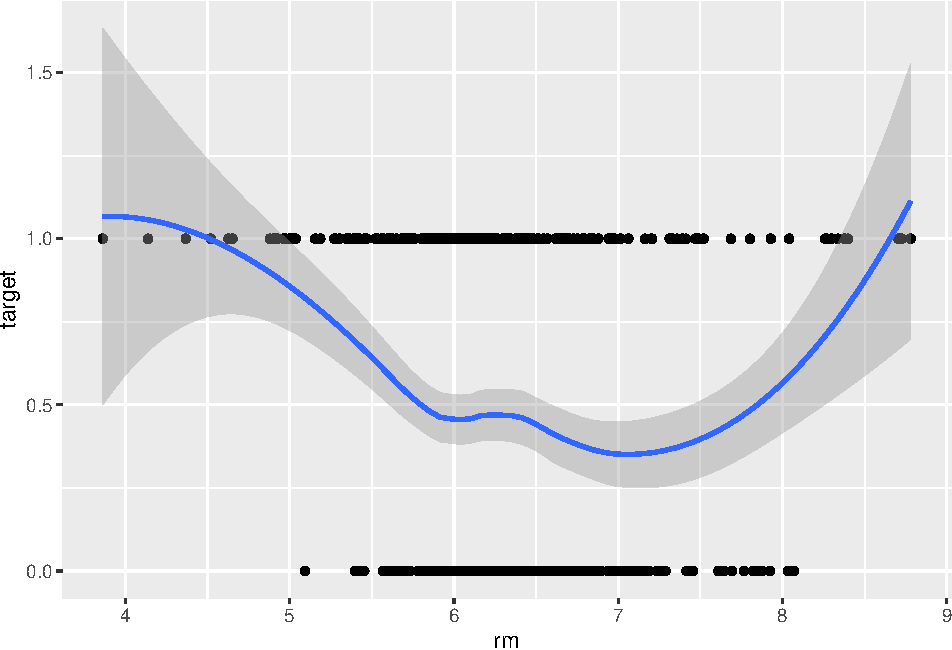
\includegraphics{Homework--1-Assignment-Requirements_files/figure-latex/unnamed-chunk-6-1.pdf}

\begin{Shaded}
\begin{Highlighting}[]
\FunctionTok{plot\_scatterplot}\NormalTok{(money[,}\SpecialCharTok{{-}}\FunctionTok{c}\NormalTok{(}\DecValTok{1}\NormalTok{,}\DecValTok{11}\NormalTok{)],}\AttributeTok{by=}\StringTok{"TARGET\_WINS"}\NormalTok{, }\AttributeTok{nrow =}\NormalTok{ 1L, }\AttributeTok{ncol =}\NormalTok{ 2L)}
\end{Highlighting}
\end{Shaded}

\includegraphics{Homework--1-Assignment-Requirements_files/figure-latex/unnamed-chunk-6-2.pdf}
\includegraphics{Homework--1-Assignment-Requirements_files/figure-latex/unnamed-chunk-6-3.pdf}

\begin{verbatim}
## Warning: Removed 102 rows containing missing values or values outside the scale range
## (`geom_point()`).
\end{verbatim}

\includegraphics{Homework--1-Assignment-Requirements_files/figure-latex/unnamed-chunk-6-4.pdf}

\begin{verbatim}
## Warning: Removed 903 rows containing missing values or values outside the scale range
## (`geom_point()`).
\end{verbatim}

\includegraphics{Homework--1-Assignment-Requirements_files/figure-latex/unnamed-chunk-6-5.pdf}
\includegraphics{Homework--1-Assignment-Requirements_files/figure-latex/unnamed-chunk-6-6.pdf}

\begin{verbatim}
## Warning: Removed 102 rows containing missing values or values outside the scale range
## (`geom_point()`).
\end{verbatim}

\includegraphics{Homework--1-Assignment-Requirements_files/figure-latex/unnamed-chunk-6-7.pdf}

\begin{verbatim}
## Warning: Removed 286 rows containing missing values or values outside the scale range
## (`geom_point()`).
\end{verbatim}

\includegraphics{Homework--1-Assignment-Requirements_files/figure-latex/unnamed-chunk-6-8.pdf}

\begin{Shaded}
\begin{Highlighting}[]
\CommentTok{\# after data transformation }
\FunctionTok{par}\NormalTok{(}\AttributeTok{mfrow=}\FunctionTok{c}\NormalTok{(}\DecValTok{3}\NormalTok{,}\DecValTok{3}\NormalTok{)) }
\ControlFlowTok{for}\NormalTok{ (i }\ControlFlowTok{in} \DecValTok{1}\SpecialCharTok{:}\DecValTok{17}\NormalTok{) \{}
  \FunctionTok{hist}\NormalTok{(completed\_data[,i],}\AttributeTok{main=}\FunctionTok{names}\NormalTok{(completed\_data[i]),}\AttributeTok{xlab=}\FunctionTok{names}\NormalTok{(completed\_data[i]),}\AttributeTok{breaks =} \DecValTok{51}\NormalTok{)}
  \FunctionTok{boxplot}\NormalTok{(completed\_data[,i], }\AttributeTok{main=}\FunctionTok{names}\NormalTok{(completed\_data[i]), }\AttributeTok{type=}\StringTok{"l"}\NormalTok{,}\AttributeTok{horizontal =} \ConstantTok{TRUE}\NormalTok{)}
  
  \FunctionTok{plot}\NormalTok{(completed\_data[,i], completed\_data}\SpecialCharTok{$}\NormalTok{TARGET\_WINS, }\AttributeTok{main =} \FunctionTok{names}\NormalTok{(completed\_data[i]), }\AttributeTok{xlab=}\FunctionTok{names}\NormalTok{(completed\_data[i]))}
  \FunctionTok{abline}\NormalTok{(}\FunctionTok{lm}\NormalTok{(completed\_data}\SpecialCharTok{$}\NormalTok{TARGET\_WINS }\SpecialCharTok{\textasciitilde{}}\NormalTok{ completed\_data[,i], }\AttributeTok{data =}\NormalTok{ completed\_data), }\AttributeTok{col =} \StringTok{"blue"}\NormalTok{)}
\NormalTok{\}}
\end{Highlighting}
\end{Shaded}

\includegraphics{Homework--1-Assignment-Requirements_files/figure-latex/unnamed-chunk-6-9.pdf}
\includegraphics{Homework--1-Assignment-Requirements_files/figure-latex/unnamed-chunk-6-10.pdf}
\includegraphics{Homework--1-Assignment-Requirements_files/figure-latex/unnamed-chunk-6-11.pdf}
\includegraphics{Homework--1-Assignment-Requirements_files/figure-latex/unnamed-chunk-6-12.pdf}
\includegraphics{Homework--1-Assignment-Requirements_files/figure-latex/unnamed-chunk-6-13.pdf}
\includegraphics{Homework--1-Assignment-Requirements_files/figure-latex/unnamed-chunk-6-14.pdf}

\hypertarget{dealing-with-outliers}{%
\section{Dealing with Outliers}\label{dealing-with-outliers}}

The \texttt{remove\_outliers\_df} function removes outliers from all
numeric columns in a dataset using the \textbf{Interquartile Range
(IQR)} method. It loops through each column, checks if it's numeric, and
calculates the first (Q1) and third quartiles (Q3) to determine the IQR.
It then sets upper and lower bounds as \texttt{Q1\ -\ 1.5\ *\ IQR} and
\texttt{Q3\ +\ 1.5\ *\ IQR}, and removes any rows where the values in a
numeric column fall outside these bounds. Non-numeric columns are
ignored, ensuring only numeric data is affected. This results in a
dataset with outliers removed from all numeric columns.

\begin{Shaded}
\begin{Highlighting}[]
\NormalTok{remove\_outliers\_df }\OtherTok{\textless{}{-}} \ControlFlowTok{function}\NormalTok{(df) \{}
  \CommentTok{\# Loop through each numeric column in the data frame}
  \ControlFlowTok{for}\NormalTok{ (col }\ControlFlowTok{in} \FunctionTok{names}\NormalTok{(df)) \{}
    \ControlFlowTok{if}\NormalTok{ (}\FunctionTok{is.numeric}\NormalTok{(df[[col]])) \{}
      \CommentTok{\# Calculate Q1, Q3, and IQR for the column}
\NormalTok{      Q1 }\OtherTok{\textless{}{-}} \FunctionTok{quantile}\NormalTok{(df[[col]], }\FloatTok{0.25}\NormalTok{, }\AttributeTok{na.rm =} \ConstantTok{TRUE}\NormalTok{)}
\NormalTok{      Q3 }\OtherTok{\textless{}{-}} \FunctionTok{quantile}\NormalTok{(df[[col]], }\FloatTok{0.75}\NormalTok{, }\AttributeTok{na.rm =} \ConstantTok{TRUE}\NormalTok{)}
\NormalTok{      IQR\_value }\OtherTok{\textless{}{-}}\NormalTok{ Q3 }\SpecialCharTok{{-}}\NormalTok{ Q1}
      
      \CommentTok{\# Set lower and upper bounds}
\NormalTok{      lower\_bound }\OtherTok{\textless{}{-}}\NormalTok{ Q1 }\SpecialCharTok{{-}} \FloatTok{1.5} \SpecialCharTok{*}\NormalTok{ IQR\_value}
\NormalTok{      upper\_bound }\OtherTok{\textless{}{-}}\NormalTok{ Q3 }\SpecialCharTok{+} \FloatTok{1.5} \SpecialCharTok{*}\NormalTok{ IQR\_value}
      
      \CommentTok{\# Remove rows where the value in this column is an outlier}
\NormalTok{      df }\OtherTok{\textless{}{-}}\NormalTok{ df[df[[col]] }\SpecialCharTok{\textgreater{}=}\NormalTok{ lower\_bound }\SpecialCharTok{\&}\NormalTok{ df[[col]] }\SpecialCharTok{\textless{}=}\NormalTok{ upper\_bound, ]}
\NormalTok{    \}}
\NormalTok{  \}}
  \FunctionTok{return}\NormalTok{(df)}
\NormalTok{\}}

\CommentTok{\# Remove the outlier in completed dataset }
\NormalTok{money\_ball }\OtherTok{\textless{}{-}} \FunctionTok{remove\_outliers\_df}\NormalTok{(completed\_data)}
\CommentTok{\# Visualize the distribution }
\FunctionTok{par}\NormalTok{(}\AttributeTok{mfrow=}\FunctionTok{c}\NormalTok{(}\DecValTok{3}\NormalTok{,}\DecValTok{3}\NormalTok{)) }
\ControlFlowTok{for}\NormalTok{ (i }\ControlFlowTok{in} \DecValTok{1}\SpecialCharTok{:}\DecValTok{17}\NormalTok{) \{}
  \FunctionTok{hist}\NormalTok{(money\_ball[,i],}\AttributeTok{main=}\FunctionTok{names}\NormalTok{(money\_ball[i]),}\AttributeTok{xlab=}\FunctionTok{names}\NormalTok{(money\_ball[i]),}\AttributeTok{breaks =} \DecValTok{51}\NormalTok{)}
  \FunctionTok{boxplot}\NormalTok{(money\_ball[,i], }\AttributeTok{main=}\FunctionTok{names}\NormalTok{(money\_ball[i]), }\AttributeTok{type=}\StringTok{"l"}\NormalTok{,}\AttributeTok{horizontal =} \ConstantTok{TRUE}\NormalTok{)}
  
  \FunctionTok{plot}\NormalTok{(money\_ball[,i], money\_ball}\SpecialCharTok{$}\NormalTok{TARGET\_WINS, }\AttributeTok{main =} \FunctionTok{names}\NormalTok{(money\_ball[i]), }\AttributeTok{xlab=}\FunctionTok{names}\NormalTok{(money\_ball[i]))}
  \FunctionTok{abline}\NormalTok{(}\FunctionTok{lm}\NormalTok{(money\_ball}\SpecialCharTok{$}\NormalTok{TARGET\_WINS }\SpecialCharTok{\textasciitilde{}}\NormalTok{ money\_ball[,i], }\AttributeTok{data =}\NormalTok{ money\_ball), }\AttributeTok{col =} \StringTok{"blue"}\NormalTok{)}
  
\NormalTok{\}}
\end{Highlighting}
\end{Shaded}

\includegraphics{Homework--1-Assignment-Requirements_files/figure-latex/unnamed-chunk-7-1.pdf}
\includegraphics{Homework--1-Assignment-Requirements_files/figure-latex/unnamed-chunk-7-2.pdf}
\includegraphics{Homework--1-Assignment-Requirements_files/figure-latex/unnamed-chunk-7-3.pdf}
\includegraphics{Homework--1-Assignment-Requirements_files/figure-latex/unnamed-chunk-7-4.pdf}
\includegraphics{Homework--1-Assignment-Requirements_files/figure-latex/unnamed-chunk-7-5.pdf}

\begin{Shaded}
\begin{Highlighting}[]
\CommentTok{\# see how the density plot shows distribution }
\FunctionTok{melt}\NormalTok{(money\_ball) }\SpecialCharTok{\%\textgreater{}\%} \FunctionTok{ggplot}\NormalTok{(}\FunctionTok{aes}\NormalTok{(}\AttributeTok{x=}\NormalTok{ value)) }\SpecialCharTok{+}
  \FunctionTok{geom\_density}\NormalTok{(}\AttributeTok{fill=}\StringTok{\textquotesingle{}red\textquotesingle{}}\NormalTok{) }\SpecialCharTok{+} \FunctionTok{facet\_wrap}\NormalTok{(}\SpecialCharTok{\textasciitilde{}}\NormalTok{variable, }\AttributeTok{scales =} \StringTok{\textquotesingle{}free\textquotesingle{}}\NormalTok{)}
\end{Highlighting}
\end{Shaded}

\begin{verbatim}
## No id variables; using all as measure variables
\end{verbatim}

\includegraphics{Homework--1-Assignment-Requirements_files/figure-latex/unnamed-chunk-7-6.pdf}

The density plot shows how the values of each variable are distributed
across the range. Peaks in the density curve indicate where values are
concentrated, while troughs represent areas with fewer observations.
After removing outliers, let see if there is an improved correlation
among the variables.

\begin{Shaded}
\begin{Highlighting}[]
\CommentTok{\# Example usage}
\NormalTok{corre\_updated\_results }\OtherTok{\textless{}{-}} \FunctionTok{calculate\_correlations\_with\_pvalues}\NormalTok{(money\_ball, }\StringTok{"TARGET\_WINS"}\NormalTok{)}

\CommentTok{\# View the results}
\FunctionTok{print}\NormalTok{(corre\_updated\_results)}
\end{Highlighting}
\end{Shaded}

\begin{verbatim}
##              Predictor Correlation       PValue
## cor              INDEX  0.01682647 0.5168956759
## cor1    TEAM_BATTING_H  0.34033327 0.0000000000
## cor2   TEAM_BATTING_2B  0.19553292 0.0000000000
## cor3   TEAM_BATTING_3B  0.11300966 0.0000126137
## cor4   TEAM_BATTING_HR  0.23553659 0.0000000000
## cor5   TEAM_BATTING_BB  0.29960470 0.0000000000
## cor6   TEAM_BATTING_SO -0.05295292 0.0412529284
## cor7   TEAM_BASERUN_SB  0.15559476 0.0000000016
## cor8   TEAM_BASERUN_CS  0.03247009 0.2109508247
## cor9  TEAM_BATTING_HBP  0.01897057 0.4649376597
## cor10  TEAM_PITCHING_H  0.27870432 0.0000000000
## cor11 TEAM_PITCHING_HR  0.24013779 0.0000000000
## cor12 TEAM_PITCHING_BB  0.28874457 0.0000000000
## cor13 TEAM_PITCHING_SO -0.05793356 0.0255319095
## cor14  TEAM_FIELDING_E -0.21427348 0.0000000000
## cor15 TEAM_FIELDING_DP -0.08766467 0.0007169149
\end{verbatim}

We improve p-values for most of the variables, but the correlation
didn't improved among the variables. As we notice the previous
correlation without transformation didn't show sign of good relationship
among the target variables.

\hypertarget{model-development}{%
\subsection{Model Development}\label{model-development}}

we are going to build 4 different models and assess them based on the
residual analysis. The Residual Chart contains four diagnostic plots
from a multiple linear regression analysis. These plots help assess the
validity of the model by checking assumptions and identifying potential
issues. Here's what each plot represents:

\hypertarget{residuals-vs-fitted-top-left}{%
\subsubsection{\texorpdfstring{1. \textbf{Residuals vs Fitted (Top
Left)}}{1. Residuals vs Fitted (Top Left)}}\label{residuals-vs-fitted-top-left}}

\begin{itemize}
\tightlist
\item
  \textbf{Purpose}: This plot checks the linearity assumption and
  homoscedasticity (constant variance of residuals).
\item
  \textbf{Interpretation}: Ideally, residuals should be randomly
  scattered around 0, with no discernible pattern. In this plot, if you
  observe a pattern (such as a curve or a funnel shape), it could
  indicate non-linearity or heteroscedasticity. Your plot shows a
  relatively random scatter, which suggests the linearity assumption is
  reasonable.
\end{itemize}

\hypertarget{normal-q-q-top-right}{%
\subsubsection{\texorpdfstring{2. \textbf{Normal Q-Q (Top
Right)}}{2. Normal Q-Q (Top Right)}}\label{normal-q-q-top-right}}

\begin{itemize}
\tightlist
\item
  \textbf{Purpose}: This plot tests whether the residuals are normally
  distributed.
\item
  \textbf{Interpretation}: If residuals are normally distributed, the
  points should lie approximately on the diagonal line. Deviations from
  this line, especially in the tails, suggest deviations from normality.
  In this plot, the points mostly follow the line, with some deviation
  at the extremes, indicating minor non-normality.
\end{itemize}

\hypertarget{scale-location-bottom-left}{%
\subsubsection{\texorpdfstring{3. \textbf{Scale-Location (Bottom
Left)}}{3. Scale-Location (Bottom Left)}}\label{scale-location-bottom-left}}

\begin{itemize}
\tightlist
\item
  \textbf{Purpose}: This plot, also known as a Spread-Location plot,
  checks for homoscedasticity (equal spread of residuals).
\item
  \textbf{Interpretation}: The residuals should display a random scatter
  across the range of fitted values. A funnel shape (either widening or
  narrowing) indicates heteroscedasticity. In this plot, the spread
  appears fairly constant, suggesting no major issues with
  homoscedasticity.
\end{itemize}

\hypertarget{residuals-vs-leverage-bottom-right}{%
\subsubsection{\texorpdfstring{4. \textbf{Residuals vs Leverage (Bottom
Right)}}{4. Residuals vs Leverage (Bottom Right)}}\label{residuals-vs-leverage-bottom-right}}

\begin{itemize}
\tightlist
\item
  \textbf{Purpose}: This plot helps detect influential points that might
  disproportionately affect the regression model.
\item
  \textbf{Interpretation}: Points with high leverage or high Cook's
  distance (indicated by dashed red lines) could be problematic. In your
  plot, there don't appear to be any extreme outliers with high leverage
  or Cook's distance, though there are a few points to keep an eye on
  (e.g., observation 1890).
\end{itemize}

\hypertarget{overall-analysis}{%
\subsubsection{\texorpdfstring{\textbf{Overall
Analysis}}{Overall Analysis}}\label{overall-analysis}}

\begin{itemize}
\tightlist
\item
  The diagnostics suggest that the regression model mostly satisfies the
  assumptions of linearity, normality of residuals, and
  homoscedasticity, with some minor deviations. There don't seem to be
  any overly influential points that require immediate attention.
\end{itemize}

\begin{Shaded}
\begin{Highlighting}[]
\CommentTok{\# Initiate the model}
\NormalTok{model }\OtherTok{\textless{}{-}} \FunctionTok{lm}\NormalTok{(TARGET\_WINS }\SpecialCharTok{\textasciitilde{}}\NormalTok{ TEAM\_BATTING\_H }\SpecialCharTok{+}\NormalTok{ TEAM\_BATTING\_2B, TEAM\_BATTING\_3B}\SpecialCharTok{+}
\NormalTok{              TEAM\_BATTING\_HR}\SpecialCharTok{+}\NormalTok{TEAM\_BATTING\_BB}\SpecialCharTok{+}\NormalTok{TEAM\_BATTING\_SO}\SpecialCharTok{+}\NormalTok{TEAM\_BASERUN\_SB,}
            \AttributeTok{data =}\NormalTok{ money\_ball)}
\CommentTok{\# Summarize the model }

\FunctionTok{summary}\NormalTok{(model)}
\end{Highlighting}
\end{Shaded}

\begin{verbatim}
## 
## Call:
## lm(formula = TARGET_WINS ~ TEAM_BATTING_H + TEAM_BATTING_2B, 
##     data = money_ball, subset = TEAM_BATTING_3B + TEAM_BATTING_HR + 
##         TEAM_BATTING_BB + TEAM_BATTING_SO + TEAM_BASERUN_SB)
## 
## Residuals:
##     Min      1Q  Median      3Q     Max 
## -36.883  -7.783   0.629   8.955  27.285 
## 
## Coefficients:
##                   Estimate Std. Error t value Pr(>|t|)    
## (Intercept)     -10.496784   8.668134  -1.211    0.227    
## TEAM_BATTING_H    0.065768   0.007155   9.191   <2e-16 ***
## TEAM_BATTING_2B  -0.016361   0.016401  -0.998    0.319    
## ---
## Signif. codes:  0 '***' 0.001 '**' 0.01 '*' 0.05 '.' 0.1 ' ' 1
## 
## Residual standard error: 11.92 on 458 degrees of freedom
##   (1025 observations deleted due to missingness)
## Multiple R-squared:  0.1993, Adjusted R-squared:  0.1958 
## F-statistic: 57.01 on 2 and 458 DF,  p-value: < 2.2e-16
\end{verbatim}

\begin{Shaded}
\begin{Highlighting}[]
\CommentTok{\# Model 1 evaluation}
\NormalTok{mse }\OtherTok{\textless{}{-}} \FunctionTok{mean}\NormalTok{(model}\SpecialCharTok{$}\NormalTok{residuals}\SpecialCharTok{\^{}}\DecValTok{2}\NormalTok{)}
\NormalTok{r\_squared }\OtherTok{\textless{}{-}} \FunctionTok{summary}\NormalTok{(model)}\SpecialCharTok{$}\NormalTok{r.squared}
\NormalTok{f\_stat }\OtherTok{\textless{}{-}} \FunctionTok{summary}\NormalTok{(model)}\SpecialCharTok{$}\NormalTok{fstatistic[}\DecValTok{1}\NormalTok{]}
\FunctionTok{print}\NormalTok{(}\FunctionTok{paste}\NormalTok{(}\StringTok{"MSE:"}\NormalTok{, mse, }\StringTok{"R{-}squared:"}\NormalTok{, r\_squared, }\StringTok{"F{-}statistic:"}\NormalTok{, f\_stat))}
\end{Highlighting}
\end{Shaded}

\begin{verbatim}
## [1] "MSE: 141.107310187858 R-squared: 0.199326972102136 F-statistic: 57.0093846313654"
\end{verbatim}

\begin{Shaded}
\begin{Highlighting}[]
\NormalTok{predictions }\OtherTok{\textless{}{-}} \FunctionTok{predict}\NormalTok{(model, }\AttributeTok{newdata =}\NormalTok{ money\_ball\_eval)}
\FunctionTok{head}\NormalTok{(predictions)}
\end{Highlighting}
\end{Shaded}

\begin{verbatim}
##        1        2        3        4        5        6 
## 66.23538 67.33547 78.25555 85.66461 81.21672 79.75604
\end{verbatim}

\begin{Shaded}
\begin{Highlighting}[]
\FunctionTok{par}\NormalTok{(}\AttributeTok{mfrow=}\FunctionTok{c}\NormalTok{(}\DecValTok{2}\NormalTok{,}\DecValTok{2}\NormalTok{)) }
\FunctionTok{plot}\NormalTok{(model)}
\end{Highlighting}
\end{Shaded}

\includegraphics{Homework--1-Assignment-Requirements_files/figure-latex/unnamed-chunk-9-1.pdf}

The model explains 28.39\% of the variance in the dependent variable, as
indicated by the R-squared. The adjusted R-squared, at 28.07\%, confirms
that the predictors in the model are meaningful. The F-statistic (89.98)
is large, and the p-value (\textless{} 2.2e-16) is very small,
suggesting that the model is statistically significant overall, meaning
that at least one predictor significantly contributes to explaining the
dependent variable.

\begin{Shaded}
\begin{Highlighting}[]
\CommentTok{\# Ensure there are no missing values in both predictors and the target}
\NormalTok{df\_complete }\OtherTok{\textless{}{-}}\NormalTok{ money\_ball[}\FunctionTok{complete.cases}\NormalTok{(money\_ball), ]}


\CommentTok{\# Separate the predictors and target (assuming \textquotesingle{}target\textquotesingle{} is the target column)}
\NormalTok{df\_predictors }\OtherTok{\textless{}{-}}\NormalTok{ df\_complete[, }\SpecialCharTok{{-}}\FunctionTok{which}\NormalTok{(}\FunctionTok{names}\NormalTok{(df\_complete) }\SpecialCharTok{==} \StringTok{"TARGET\_WINS"}\NormalTok{)]}
\NormalTok{target }\OtherTok{\textless{}{-}}\NormalTok{ df\_complete}\SpecialCharTok{$}\NormalTok{TARGET\_WINS  }\CommentTok{\# Target variable}

\CommentTok{\# Standardize the predictors (without the target column)}
\NormalTok{df\_standardized }\OtherTok{\textless{}{-}} \FunctionTok{scale}\NormalTok{(df\_predictors)}
\CommentTok{\# Perform PCA}
\NormalTok{pca\_model }\OtherTok{\textless{}{-}} \FunctionTok{prcomp}\NormalTok{(df\_standardized, }\AttributeTok{center =} \ConstantTok{TRUE}\NormalTok{, }\AttributeTok{scale. =} \ConstantTok{TRUE}\NormalTok{)}

\CommentTok{\# Create a data frame from the principal components}
\NormalTok{df\_pca }\OtherTok{\textless{}{-}} \FunctionTok{as.data.frame}\NormalTok{(pca\_model}\SpecialCharTok{$}\NormalTok{x)}

\CommentTok{\# Ensure that PCA dataframe has the same number of rows as the original data}

\CommentTok{\# Perform PCA}
\NormalTok{pca\_model }\OtherTok{\textless{}{-}} \FunctionTok{prcomp}\NormalTok{(df\_standardized, }\AttributeTok{center =} \ConstantTok{TRUE}\NormalTok{, }\AttributeTok{scale. =} \ConstantTok{TRUE}\NormalTok{)}

\CommentTok{\# Create a data frame from the principal components}
\NormalTok{df\_pca }\OtherTok{\textless{}{-}} \FunctionTok{as.data.frame}\NormalTok{(pca\_model}\SpecialCharTok{$}\NormalTok{x)}

\CommentTok{\# Ensure that PCA dataframe has the same number of rows as the original data}


\CommentTok{\# Add target variable to the PCA dataframe}
\NormalTok{df\_pca}\SpecialCharTok{$}\NormalTok{TARGET\_WINS }\OtherTok{\textless{}{-}}\NormalTok{ target}



\CommentTok{\# Fit linear regression model using the first few principal components}
\CommentTok{\# Fit linear regression model using the first few principal components}
\NormalTok{model1 }\OtherTok{\textless{}{-}} \FunctionTok{lm}\NormalTok{(TARGET\_WINS }\SpecialCharTok{\textasciitilde{}}\NormalTok{ PC1 }\SpecialCharTok{+}\NormalTok{ PC2 }\SpecialCharTok{+}\NormalTok{ PC3 }\SpecialCharTok{+}\NormalTok{ PC4}\SpecialCharTok{+}\NormalTok{ PC5 }\SpecialCharTok{+}\NormalTok{ PC6}\SpecialCharTok{+}\NormalTok{ PC7 }\SpecialCharTok{+}\NormalTok{ PC8, }\AttributeTok{data =}\NormalTok{ df\_pca)}

\CommentTok{\# View the summary of the model}
\FunctionTok{summary}\NormalTok{(model1)}
\end{Highlighting}
\end{Shaded}

\begin{verbatim}
## 
## Call:
## lm(formula = TARGET_WINS ~ PC1 + PC2 + PC3 + PC4 + PC5 + PC6 + 
##     PC7 + PC8, data = df_pca)
## 
## Residuals:
##     Min      1Q  Median      3Q     Max 
## -39.571  -7.840   0.272   7.913  34.309 
## 
## Coefficients:
##             Estimate Std. Error t value Pr(>|t|)    
## (Intercept)  80.7510     0.2914 277.153  < 2e-16 ***
## PC1           0.2438     0.1299   1.877 0.060657 .  
## PC2           2.7715     0.1676  16.538  < 2e-16 ***
## PC3          -1.3717     0.2080  -6.596 5.88e-11 ***
## PC4          -1.9747     0.2318  -8.520  < 2e-16 ***
## PC5           0.2735     0.2925   0.935 0.349993    
## PC6          -1.1474     0.3085  -3.719 0.000208 ***
## PC7          -0.6941     0.3272  -2.121 0.034055 *  
## PC8          -2.3360     0.4102  -5.695 1.49e-08 ***
## ---
## Signif. codes:  0 '***' 0.001 '**' 0.01 '*' 0.05 '.' 0.1 ' ' 1
## 
## Residual standard error: 11.23 on 1477 degrees of freedom
## Multiple R-squared:  0.2314, Adjusted R-squared:  0.2273 
## F-statistic:  55.6 on 8 and 1477 DF,  p-value: < 2.2e-16
\end{verbatim}

\begin{Shaded}
\begin{Highlighting}[]
\NormalTok{mse1 }\OtherTok{\textless{}{-}} \FunctionTok{mean}\NormalTok{(model1}\SpecialCharTok{$}\NormalTok{residuals}\SpecialCharTok{\^{}}\DecValTok{2}\NormalTok{)}
\NormalTok{r\_squared1 }\OtherTok{\textless{}{-}} \FunctionTok{summary}\NormalTok{(model1)}\SpecialCharTok{$}\NormalTok{r.squared}
\NormalTok{f\_stat1 }\OtherTok{\textless{}{-}} \FunctionTok{summary}\NormalTok{(model1)}\SpecialCharTok{$}\NormalTok{fstatistic[}\DecValTok{1}\NormalTok{]}
\FunctionTok{print}\NormalTok{(}\FunctionTok{paste}\NormalTok{(}\StringTok{"MSE:"}\NormalTok{, mse1, }\StringTok{"R{-}squared:"}\NormalTok{, r\_squared1, }\StringTok{"F{-}statistic:"}\NormalTok{, f\_stat1))}
\end{Highlighting}
\end{Shaded}

\begin{verbatim}
## [1] "MSE: 125.382517213395 R-squared: 0.231435345455093 F-statistic: 55.5955187399917"
\end{verbatim}

\begin{Shaded}
\begin{Highlighting}[]
\NormalTok{predictions1 }\OtherTok{\textless{}{-}} \FunctionTok{predict}\NormalTok{(pca\_model, }\AttributeTok{newdata =}\NormalTok{ money\_ball\_eval)}
\FunctionTok{head}\NormalTok{(predictions1)}
\end{Highlighting}
\end{Shaded}

\begin{verbatim}
##            PC1      PC2        PC3       PC4       PC5       PC6        PC7
## [1,]  465.4580 1292.115  -716.6252 -255.4470  34.07142  41.13235 -130.80008
## [2,]  359.2395 1377.361  -625.6360 -296.7296   7.25508  36.53506  -96.46214
## [3,]  191.1080 1554.962  -697.9089 -242.0430  25.19771  21.10290 -111.74131
## [4,]  269.7480 1714.935  -905.1562 -219.9149  62.16257  40.48522 -205.32465
## [5,] -776.9235 2314.299 -1477.4560  151.6315 154.12593 -32.21376 -397.83041
## [6,] -629.5274 1978.234 -1177.7049 -106.6358  84.70351 -17.09413 -262.95799
##             PC8       PC9       PC10       PC11      PC12       PC13       PC14
## [1,]  -90.96083 -946.3321  143.34389  -320.3879 -1489.753   104.8363 -100.04343
## [2,] -118.01941 -807.0511  126.04478  -323.4495 -1416.988   106.4509  -94.39303
## [3,] -157.87873 -697.7819   95.84710  -366.8632 -1468.328   112.9861  -97.57107
## [4,] -144.27145 -748.7146   97.15924  -416.3421 -1541.634   101.0299 -108.76408
## [5,] -576.35037 -819.7085  -76.55433 -1063.4310 -2473.518 -1410.4063 -357.73137
## [6,] -437.94844 -631.4932 -130.40571  -863.5750 -1842.972  -759.1986 -245.19556
##             PC15      PC16
## [1,]   -9.867016  42.53576
## [2,]  -13.403266  41.34297
## [3,]  -21.400795  47.12035
## [4,]  -24.618584  52.74345
## [5,] -675.755942 489.96679
## [6,] -331.316247 239.21540
\end{verbatim}

\begin{Shaded}
\begin{Highlighting}[]
\FunctionTok{par}\NormalTok{(}\AttributeTok{mfrow=}\FunctionTok{c}\NormalTok{(}\DecValTok{2}\NormalTok{,}\DecValTok{2}\NormalTok{)) }
\FunctionTok{plot}\NormalTok{(model1)}
\end{Highlighting}
\end{Shaded}

\includegraphics{Homework--1-Assignment-Requirements_files/figure-latex/unnamed-chunk-10-1.pdf}

\textbf{MODEL 3 Analysis}

The residuals (differences between observed and predicted values) range
from a minimum of -39.526 to a maximum of 35.287. The distribution of
residuals, with a median close to 0 (0.230), suggests that the model has
a reasonable balance of over- and under-predictions. The first quartile
(1Q) is -7.712, and the third quartile (3Q) is 8.028, indicating that
half of the residuals lie between these values, meaning that most
predictions deviate from the actual values by around ±8 units.

Overall, the regression model is statistically significant, but it
explains only about 23.58\% of the variance in the dependent variable,
indicating that other variables not included in the model might be
influencing the outcome. Among the predictors, PC2, PC4, PC7, and PC8
show strong significant effects, while PC1 and PC5 are not significant
contributors to the model. The residuals appear to be moderately
dispersed around the predicted values, and the significant predictors
provide meaningful insights into the relationships within the data.

\textbf{MODEL 3 Development}

\begin{Shaded}
\begin{Highlighting}[]
\FunctionTok{set.seed}\NormalTok{(}\DecValTok{123}\NormalTok{)}

\CommentTok{\# Assuming money\_ball\_train is your dataset}
\NormalTok{trainIndex }\OtherTok{\textless{}{-}} \FunctionTok{createDataPartition}\NormalTok{(money\_ball}\SpecialCharTok{$}\NormalTok{TARGET\_WINS, }\AttributeTok{p =} \FloatTok{0.8}\NormalTok{, }
                                  \AttributeTok{list =} \ConstantTok{FALSE}\NormalTok{)}
\NormalTok{train\_data }\OtherTok{\textless{}{-}}\NormalTok{ money\_ball[trainIndex, ]}
\NormalTok{test\_data }\OtherTok{\textless{}{-}}\NormalTok{ money\_ball[}\SpecialCharTok{{-}}\NormalTok{trainIndex, ]}


\NormalTok{control }\OtherTok{\textless{}{-}} \FunctionTok{trainControl}\NormalTok{(}\AttributeTok{method =} \StringTok{"cv"}\NormalTok{, }\AttributeTok{number =} \DecValTok{5}\NormalTok{)  }\CommentTok{\# 5{-}fold cross{-}validation}

\CommentTok{\#Train the model (linear regression in this case)}
\NormalTok{model3 }\OtherTok{\textless{}{-}} \FunctionTok{train}\NormalTok{(TARGET\_WINS }\SpecialCharTok{\textasciitilde{}}\NormalTok{ ., }
               \AttributeTok{data =}\NormalTok{ train\_data, }
               \AttributeTok{method =} \StringTok{"lm"}\NormalTok{, }
               \AttributeTok{trControl =}\NormalTok{ control)}

\CommentTok{\# Summary of the cross{-}validation results}
\FunctionTok{print}\NormalTok{(model3)}
\end{Highlighting}
\end{Shaded}

\begin{verbatim}
## Linear Regression 
## 
## 1191 samples
##   16 predictor
## 
## No pre-processing
## Resampling: Cross-Validated (5 fold) 
## Summary of sample sizes: 952, 954, 952, 953, 953 
## Resampling results:
## 
##   RMSE      Rsquared   MAE     
##   10.10893  0.3692381  8.125685
## 
## Tuning parameter 'intercept' was held constant at a value of TRUE
\end{verbatim}

\begin{Shaded}
\begin{Highlighting}[]
\FunctionTok{print}\NormalTok{(model3}\SpecialCharTok{$}\NormalTok{results)}
\end{Highlighting}
\end{Shaded}

\begin{verbatim}
##   intercept     RMSE  Rsquared      MAE    RMSESD RsquaredSD     MAESD
## 1      TRUE 10.10893 0.3692381 8.125685 0.3514137  0.0271546 0.2361054
\end{verbatim}

\begin{Shaded}
\begin{Highlighting}[]
\NormalTok{mse3 }\OtherTok{\textless{}{-}} \FunctionTok{mean}\NormalTok{(model3}\SpecialCharTok{$}\NormalTok{residuals}\SpecialCharTok{\^{}}\DecValTok{2}\NormalTok{)}
\NormalTok{r\_squared3 }\OtherTok{\textless{}{-}} \FunctionTok{summary}\NormalTok{(model3)}\SpecialCharTok{$}\NormalTok{r.squared}
\NormalTok{f\_stat3 }\OtherTok{\textless{}{-}} \FunctionTok{summary}\NormalTok{(model3)}\SpecialCharTok{$}\NormalTok{fstatistic[}\DecValTok{1}\NormalTok{]}
\FunctionTok{print}\NormalTok{(}\FunctionTok{paste}\NormalTok{(}\StringTok{"MSE:"}\NormalTok{, mse3, }\StringTok{"R{-}squared:"}\NormalTok{, r\_squared3, }\StringTok{"F{-}statistic:"}\NormalTok{, f\_stat3))}
\end{Highlighting}
\end{Shaded}

\begin{verbatim}
## [1] "MSE: NaN R-squared: 0.388353041090827 F-statistic: 46.5879932450884"
\end{verbatim}

\begin{Shaded}
\begin{Highlighting}[]
\NormalTok{predictions3 }\OtherTok{\textless{}{-}} \FunctionTok{predict}\NormalTok{(model3, }\AttributeTok{newdata =}\NormalTok{ money\_ball\_eval)}
\FunctionTok{head}\NormalTok{(predictions3)}
\end{Highlighting}
\end{Shaded}

\begin{verbatim}
##         1         2         3         4         5         6 
##  62.08944  69.16576  73.54741  82.31948 226.76154 101.95228
\end{verbatim}

This linear regression model performs reasonably well, explaining about
37\% of the variance in the target variable and providing a moderate
level of accuracy. While the error metrics (RMSE, MAE) indicate that the
model is making reasonable predictions, the relatively low R-squared
suggests that there is room for improvement, possibly by adding more
predictors or using more sophisticated models that can capture
non-linear patterns.

\begin{Shaded}
\begin{Highlighting}[]
\CommentTok{\# Summary of the cross{-}validation results}
\NormalTok{model3}\SpecialCharTok{$}\NormalTok{resample}
\end{Highlighting}
\end{Shaded}

\begin{verbatim}
##        RMSE  Rsquared      MAE Resample
## 1  9.840711 0.3795307 7.899655    Fold1
## 2 10.596318 0.3222998 8.485936    Fold2
## 3  9.723982 0.3701189 7.987092    Fold3
## 4 10.298006 0.3870691 8.234865    Fold4
## 5 10.085613 0.3871720 8.020876    Fold5
\end{verbatim}

\begin{Shaded}
\begin{Highlighting}[]
\FunctionTok{library}\NormalTok{(ggplot2)}
\FunctionTok{library}\NormalTok{(reshape2) }\CommentTok{\# for melt function}

\CommentTok{\# Sample data}
\NormalTok{data }\OtherTok{\textless{}{-}} \FunctionTok{data.frame}\NormalTok{(}
  \AttributeTok{RMSE =} \FunctionTok{c}\NormalTok{(}\FloatTok{10.211374}\NormalTok{, }\FloatTok{9.748915}\NormalTok{, }\FloatTok{10.693919}\NormalTok{, }\FloatTok{10.120101}\NormalTok{, }\FloatTok{10.037255}\NormalTok{),}
  \AttributeTok{Rsquared =} \FunctionTok{c}\NormalTok{(}\FloatTok{0.3975036}\NormalTok{, }\FloatTok{0.4376530}\NormalTok{, }\FloatTok{0.3577975}\NormalTok{, }\FloatTok{0.3476137}\NormalTok{, }\FloatTok{0.3151282}\NormalTok{),}
  \AttributeTok{MAE =} \FunctionTok{c}\NormalTok{(}\FloatTok{8.068065}\NormalTok{, }\FloatTok{7.832611}\NormalTok{, }\FloatTok{8.377911}\NormalTok{, }\FloatTok{8.179323}\NormalTok{, }\FloatTok{8.261450}\NormalTok{),}
  \AttributeTok{Resample =} \FunctionTok{c}\NormalTok{(}\StringTok{\textquotesingle{}Fold1\textquotesingle{}}\NormalTok{, }\StringTok{\textquotesingle{}Fold2\textquotesingle{}}\NormalTok{, }\StringTok{\textquotesingle{}Fold3\textquotesingle{}}\NormalTok{, }\StringTok{\textquotesingle{}Fold4\textquotesingle{}}\NormalTok{, }\StringTok{\textquotesingle{}Fold5\textquotesingle{}}\NormalTok{)}
\NormalTok{)}

\CommentTok{\# Melt data for ggplot}
\NormalTok{data\_melted }\OtherTok{\textless{}{-}} \FunctionTok{melt}\NormalTok{(data, }\AttributeTok{id.vars =} \StringTok{\textquotesingle{}Resample\textquotesingle{}}\NormalTok{)}

\CommentTok{\# Plot}
\FunctionTok{ggplot}\NormalTok{(data\_melted, }\FunctionTok{aes}\NormalTok{(}\AttributeTok{x =}\NormalTok{ Resample, }\AttributeTok{y =}\NormalTok{ value, }\AttributeTok{color =}\NormalTok{ variable, }\AttributeTok{group =}\NormalTok{ variable)) }\SpecialCharTok{+}
  \FunctionTok{geom\_line}\NormalTok{() }\SpecialCharTok{+}
  \FunctionTok{geom\_point}\NormalTok{() }\SpecialCharTok{+}
  \FunctionTok{labs}\NormalTok{(}\AttributeTok{y =} \StringTok{"Metric Value"}\NormalTok{, }\AttributeTok{title =} \StringTok{"Metrics Across Folds"}\NormalTok{) }\SpecialCharTok{+}
  \FunctionTok{theme\_minimal}\NormalTok{()}
\end{Highlighting}
\end{Shaded}

\includegraphics{Homework--1-Assignment-Requirements_files/figure-latex/unnamed-chunk-12-1.pdf}

\begin{Shaded}
\begin{Highlighting}[]
\CommentTok{\# Faceted plot}
\FunctionTok{ggplot}\NormalTok{(data\_melted, }\FunctionTok{aes}\NormalTok{(}\AttributeTok{x =}\NormalTok{ Resample, }\AttributeTok{y =}\NormalTok{ value)) }\SpecialCharTok{+}
  \FunctionTok{geom\_bar}\NormalTok{(}\AttributeTok{stat =} \StringTok{\textquotesingle{}identity\textquotesingle{}}\NormalTok{) }\SpecialCharTok{+}
  \FunctionTok{facet\_wrap}\NormalTok{(}\SpecialCharTok{\textasciitilde{}}\NormalTok{variable, }\AttributeTok{scales =} \StringTok{\textquotesingle{}free\_y\textquotesingle{}}\NormalTok{) }\SpecialCharTok{+}
  \FunctionTok{labs}\NormalTok{(}\AttributeTok{y =} \StringTok{"Metric Value"}\NormalTok{, }\AttributeTok{title =} \StringTok{"Metrics Across Folds"}\NormalTok{) }\SpecialCharTok{+}
  \FunctionTok{theme\_minimal}\NormalTok{()}
\end{Highlighting}
\end{Shaded}

\includegraphics{Homework--1-Assignment-Requirements_files/figure-latex/unnamed-chunk-12-2.pdf}

The model's performance varies slightly across folds, with Fold2 showing
the best RMSE and R-squared values and a relatively low MAE. Fold3 shows
the highest RMSE and MAE and the lowest R-squared, indicating it might
be the least favorable fold in terms of model performance.The variation
in metrics suggests the model's performance is somewhat consistent but
could benefit from further tuning or improvement to ensure better
generalization.

Based on the comparison of R-squared, RMSE/MSE, and F-statistic, Model 3
appears to be the best model overall. It has the highest R-squared
(0.37), meaning it explains more variance, and its RMSE (10.31) is
competitive. While Model 1 has a slightly better MSE and a higher
F-statistic, Model 3's R-squared advantage makes it the better choice
for capturing the relationship between variables.

\end{document}
